\documentclass[11pt]{article}
\usepackage[autonum]{macros}

% figures and bibliography
%\usepackage[sorting=nyt,backend=biber,bibstyle=alphabetic,citestyle=alphabetic]{biblatex}
%\usepackage[backend=biber]{biblatex}
\usepackage{natbib}
%\bibliography{ref.bib}


% set margins' lenghts %%%%%%
\setlength{\oddsidemargin}{0.0 in}
\setlength{\evensidemargin}{0.0 in}
\setlength{\topmargin}{-0.6 in}
\setlength{\textwidth}{6.5 in}
\setlength{\textheight}{8.5 in}
\setlength{\headsep}{0.75 in}
\setlength{\parindent}{0 in}
\setlength{\parskip}{0.1 in}

\usepackage{multirow} % for table
\usepackage[table]{xcolor} % alternating row colors in tables
\usepackage{placeins}
\renewcommand{\abstractname}{Executive Summary} % change title of abstract

% set fancy style for margins %%%%%%
\usepackage{fancyhdr}
\pagestyle{fancy}
\fancyhf{}
\lhead{Madden, C.l}
\chead{UBC STCS}
\rhead{Diluvi, G. C.}
\cfoot{\thepage}





\title{\vspace{-2cm}\Large A Statistical View of The Right to Vancouverism: Social Reproduction Placemaking in the Revanchist City}
\author{\normalsize Gian Carlo Diluvi\footnote{Department of Statistics, University of British Columbia. Contact: \href{mailto:gian.diluvi@stat.ubc.ca}{\texttt{gian.diluvi@stat.ubc.ca}}.}}
\date{\normalsize Client: Cheryl-lee Madden
\vskip 0.1cm
June 2021}




\begin{document}

\maketitle



%\begin{abstract}
%  \noindent Lorem ipsum dolor sit amet, consectetur adipisicing elit, sed do eiusmod tempor incididunt ut labore et dolore magna aliqua. Ut enim ad minim veniam, quis nostrud exercitation ullamco laboris nisi ut aliquip ex ea commodo consequat. Duis aute irure dolor in reprehenderit in voluptate velit esse cillum dolore eu fugiat nulla pariatur. Excepteur sint occaecat cupidatat non proident, sunt in culpa qui officia deserunt mollit anim id est laborum.
%\end{abstract}


\section{Introduction}

Statistics Canada just published the results of the 2018 Canadian
Household Survey \cite{chs2018}. \cite{blog} used the publicly-available
data to analyze mobility in Canada, with an emphasis on forced moves
and tenure precarity.
\\

A new research project aims at expanding the analysis \cite{blog}
to account for low-income women as well as different neighborhoods within
Vancouver. Once the 2021 CHS data become available, the project also aims
to understand the impact of the COVID-19 pandemic on low-income women
tenure precarity.
The project poses three statistical questions:
\benum
  \item whether the publicly-available data from the 2018 CHS is appropriate
  for statistical inference;
  \item whether the statistical analyses in \cite{blog} can also be applied
  to study the impact of gender and income in forced moves in Vancouver;
  \item whether the analyses of \cite{blog}, which are done at the city
  level, can be expanded to include more geographic granularity within Vancouver.
\eenum

In Section \ref{sec:stats}, we discuss the limitations of using the
publicly-available data of the 2018 CHS and how these apply to each
of the three statistical questions. In Section \ref{sec:eda}, we showcase
potential visualizations that can be used to address the statistical
questions. Section \ref{sec:conclusion} concludes the report.





\section{Statistical Considerations of the 2018 CHS PUMF} \label{sec:stats}


In order to protect the privacy of survey respondents (i.e.
preventing any respondent or household from being identified), data obtained
in the CHS is modified in various ways. \cite[Section~6]{chsguide} goes
into detail about the safeguards used by Statistics Canada. These include
decreasing the level of geographic detail; grouping answers into
categories in questions that contain many answers; adding random noise to
some quantitative variables; and rounding very small or large quantitative
values, which normally correspond to extreme (i.e. rare) households.
\\


The modified data, called the \textit{public use microdata file} (PUMF),
is then made public. Naturally, analyses based on the PUMF will differ from
those carried out using the full master file of Statistics Canada due
to the data modification process used to decrease disclosure risk.
\cite[Section~7]{chsguide} explains in detail all the limitations of analyses
based on the PUMF. Succinctly, however, the PUMF should not be used to carry out
statistical analyses. Rather, it should be used to conduct exploratory data
analyses that might indicate which models are appropriate and possibly
to obtain preliminary estimates of variables of interest.
\\

Related to the first statistical question, the PUMF cannot be reliably used
to measure variability, and it also does not include bootstrap weights.
Hence, practically any statistical test would produce invalid results.
This is because, even if point estimates are not necessarily way off
when compared with the values obtained from Statistics Canada's master file,
there is no way to reliably measure the quality of each estimate.
Furthermore, the accuracy of point estimates is inversely proportional to
the number of variables that are being cross-tabulated.
Again, however, there is no objective and reliable way to measure this accuracy.
\\

Once preliminary results have been obtained and an appropriate model
(or family of models) selected, the PUMF user guide \cite{chsguide} recommends
requesting access to the CHS master files. Statistical analyses based on
the full data files will be valid and, furthermore, can be fit
with a greater level of detail (e.g. geographically).
\\

As for the second statistical question, the PUMF contains the gender
of the reference person, i.e. the person answering the survey.
This means that accounting for gender using the PUMF would be difficult
as there is no indication of the relationship between the reference person
and the main provider of each household. It is possible that the master file
does contain information about each member of the household, including gender,
although the PUMF guide is not very clear about this.
\\

In terms of the third statistical question, the PUMF only
contains geographic information at the census metropolitan area (CMA),
which for British Columbia (B.C.) corresponds to three categories:
Vancouver, other large cities, and the rest of B.C. The confidential
master file of Statistics Canada, however, does contain more detailed
information that would allow a more granular analysis.
Specifically, analyses that include neighborhoods within Vancouver can only
be done based on the full master file.
\\

Another point of interest is that of low-income families. The PUMF contains
multiple variables related to the economical situation of each household,
such as the annual income of each household. This information can be directly
used to analyze (with the caveats mentioned in the previous paragraphs)
the situation of low-income households. However, it should be mentioned that
using poverty or low-income indices that depend on multiple variables might
be unfeasible for multiple reasons. First, it is possible that not all the
variables are available in the PUMF. Second, if they are, cross-tabulating
multiple variables can decrease the accuracy of point estimates based on
the PUMF, as was mentioned before.
\\

Finally, it is not possile to use the 2018 CHS to analyze the impact that
the COVID-19 pandemic has had on Canadian households due to the pandemic
occurring three years after the census was carried out. However, it would
be possible to use the 2021 census to study the impact of the pandemic
once it is made public, with the same considerations as mentioned above.




\section{Exploratory Data Analysis} \label{sec:eda}

In this section, we will address the second and third statistical
questions, i.e. the landscape of forced moves for low-income women
in Vancouver.
\\

As we discussed in the previous section, the PUMF contains the gender
of the reference person. We will proceed assuming that the reference
person corresponds to the primary provider of each household.
Note, however, that this assumption might very well not hold, but it
allows us to propose visualizations to understand the relationship
between gender and forced moves. We suggest repeating these figures
with the full master file of the 2018 CHS.
\\


Figure \ref{fig:fm_gender} shows that slightly more men were forced to move
out of their house, although it is not possible to assess whether the
difference is significant in light of the previous section.
Figure \ref{fig:income_gender} shows that women that were \textit{not}
forced to move tend to have a higher income than those who were.
Indeed, all the outlier points with really high incomes correspond to
women who were not forced to move.
On the other hand, the median income of women who were forced to move
is smaller, although again it is not possible to test whether this
difference is statistically significant (e.g. via a $t$-test or a
permutation test; see \cite[Ch.~9.3]{agresti} for a more detailed explanation).


\begin{figure}
  \centering
  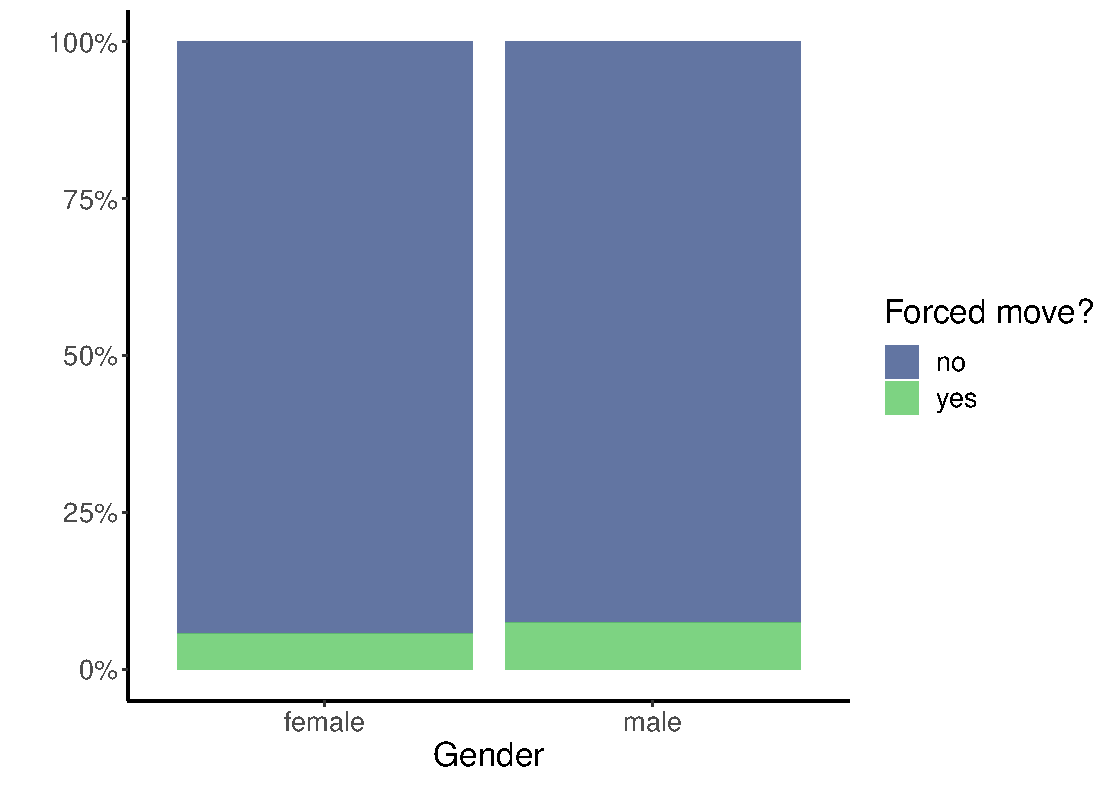
\includegraphics[scale=0.5]{fig/fm_gender.pdf}
  \caption{Percentage of people in B.C. that were forcefully moved
  from their house by gender.}
  \label{fig:fm_gender}
\end{figure}



\begin{figure}
  \centering
  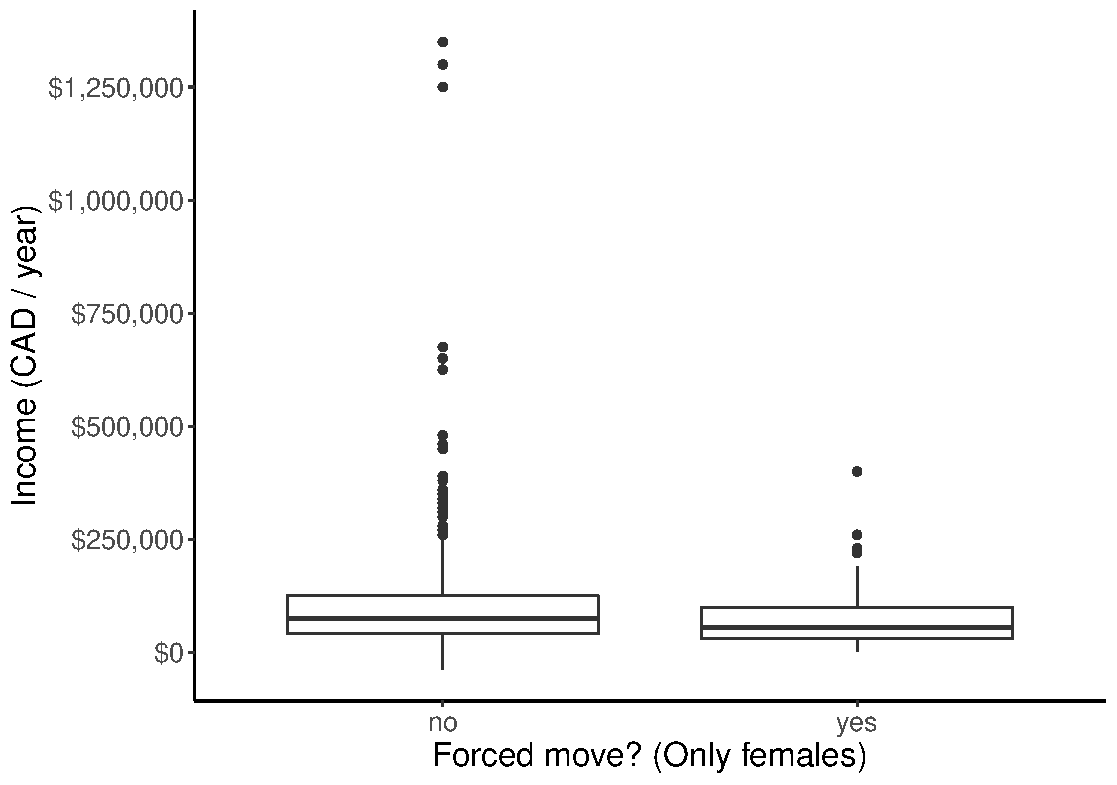
\includegraphics[scale=0.5]{fig/income_gender.pdf}
  \caption{Distribution of income of women in B.C., divided by
  whether they were forced to move from their house.}
  \label{fig:income_gender}
\end{figure}



\begin{figure}
  \centering
  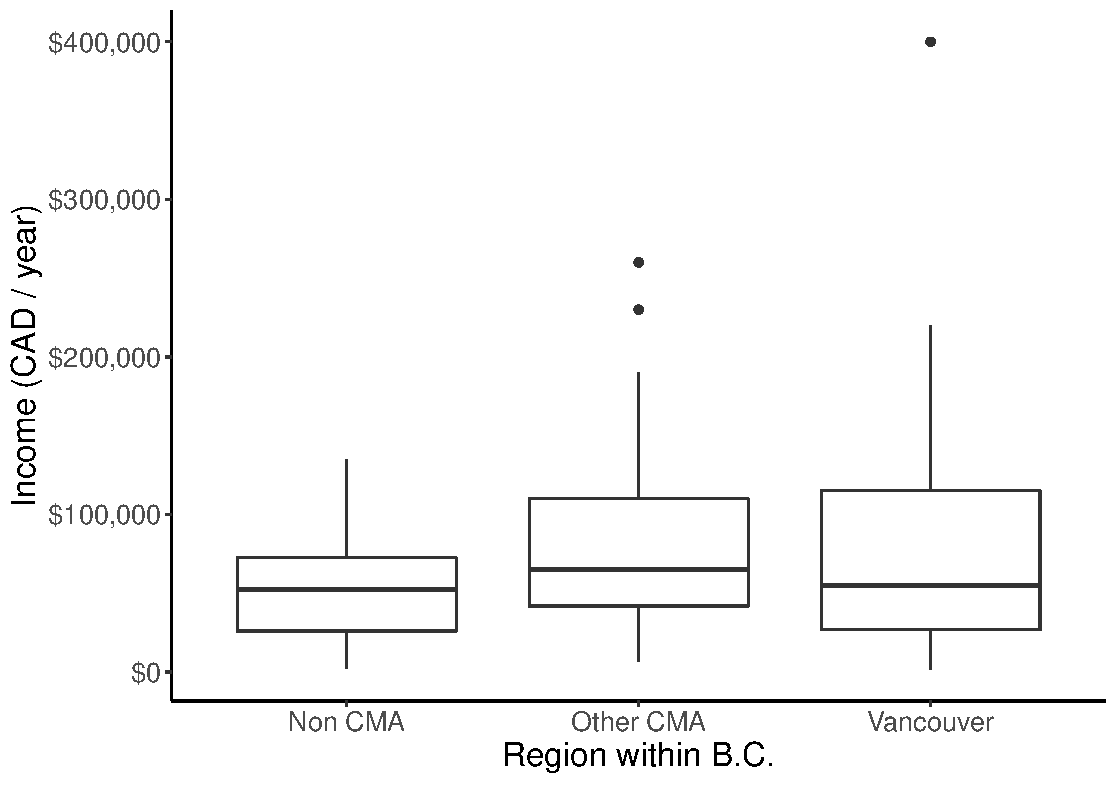
\includegraphics[scale=0.5]{fig/income_location.pdf}
  \caption{Distribution of income of women in B.C. who were forced
  to move, divided by regions within B.C.}
  \label{fig:income_location}
\end{figure}



Finally, Figure \ref{fig:income_location} shows the distribution of income
for all women in B.C. who were forced to move. All three distributions seem
similar, although the non-CMA zone has a slightly smaller range of incomes.
This is likely due to cities being more expensive (which translates to
generally higher-paying jobs). This is the finest level of detail included
in the PUMF, so it is not possible to drill down into Vancouver. As mentioned
before, the master file of Statistics Canada contains more granular information
that would allow for such an analysis to be carried out---including whether
differences between e.g. neighborhoods are statistically significant, which
can be tested via an Analysis of Variance (ANOVA) or a non-parametric
version thereof.
(See \cite[Ch.~14]{agresti} for a more detailed explanation of ANOVA.)

\FloatBarrier

\section{Conclusion} \label{sec:conclusion}


In this report, we discussed using the 2018 Canadian Household Survey
to study precarious tenure conditions in Canada. Specific emphasis
was given to adapting the analysis of \cite{blog} to low-income women
in Vancouver.
\\

First, we discussed the limitations of using the 2018 CHS PUMF.
Before being made public, the master file with the full data
is modified by Statistics Canada to prevent specificic households
from being identified.
This, combined with the fact that bootstrap weights are not made
available, prevents using the PUMF for inferential statistics.
Indeed, the PUMF user guide recommends only using the public data
for exploratory analyses and preliminary results, cross-tabulating
as little as possible.
\\

We also showcased some specific visual analyses that address the main
statistical questions, and that adapt \cite{blog} to low-income women
in B.C. Some limitations regarding the gender variable contained in the
PUMF were discussed, as were the geographic granularity limitations---namely
that there is no data available at the neighborhood level within Vancouver in
the PUMF.
\\

Once the 2021 CHS is made available, it can be used to also account for
the impact of the COVID-19 pandemic. However, given that the 2018 CHS
was published in 2021, it could very well be that the 2021 CHS is
published in 2024. Until then, it is not possible to incorporate information
related to the pandemic into analyses of tenure precarity in Canada.


\clearpage
%\printbibliography
\bibliographystyle{abbrvnat}
\bibliography{ref}


\end{document}
